\begin{frame}[label=mc_hopeful]
    \frametitle{Monte Carlo Sims: Future Work}
    \begin{columns}
        \begin{column}{0.7\textwidth}
            \alert{Generating a better meteor population} would give higher fidelity results with fewer limitations
            \begin{itemize} \footnotesize
                \item Currently: representative of the sporadic background meteor population over long times
                \item Relationships between stochastic variables is not represented
                \item More useful: a peer-reviewed meteor input function 
            \end{itemize}

            \alert{Simulating an existing multistatic networks} could help inform its expansion and provide further validation \\ ~ \\

            This tool could be used to \alert{directly estimate optimal network expansions} with the help of machine learning methods
            \begin{itemize} \footnotesize
                \item Currently: many network configurations are simulated and compared
                \item More useful: direct estimation of optimal \textcolor{blue}{\textbf{TX}}/\textcolor{red}{\textbf{RX}} location
            \end{itemize}
        \end{column}
        \begin{column}{0.4\textwidth}
            \centering
            \begin{tikzpicture}
                \node[inner sep =0] (img) {
                    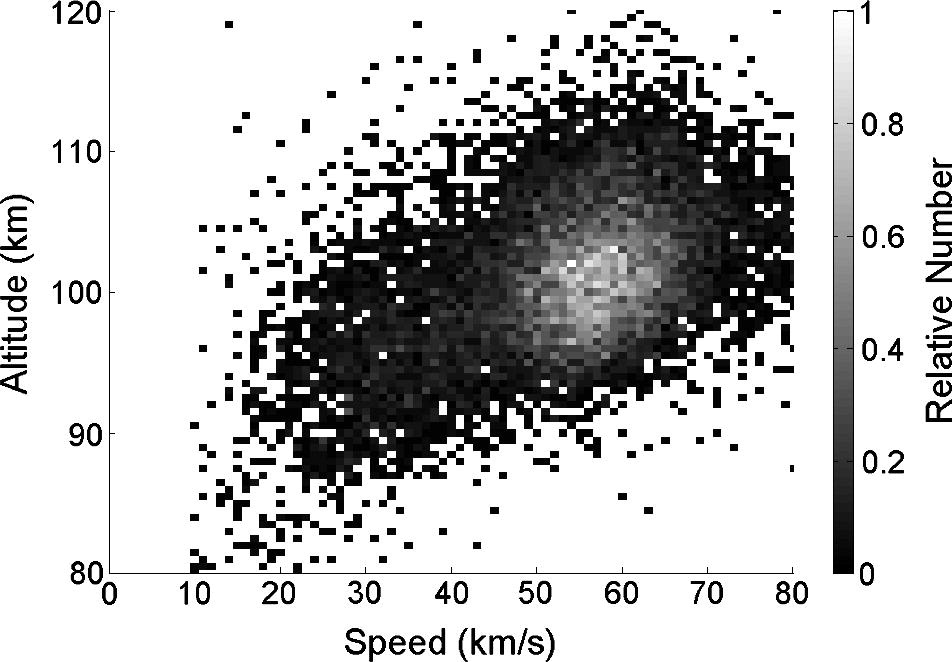
\includegraphics[height=0.4\textheight]{img/MIF_pifko.jpg}
                };
                \node[anchor = south east] at ([yshift = 0.5cm, xshift=-0.5cm]img.south east) { 
                    {\fontsize{5}{5.4}\selectfont \textcolor{black}{Credit: \citeauthor{pifko_MeteoroidInputFunction_2013}, \citeyear{pifko_MeteoroidInputFunction_2013} \cite{pifko_MeteoroidInputFunction_2013}}}
                };
            \end{tikzpicture}
            \vspace{0.2cm}
            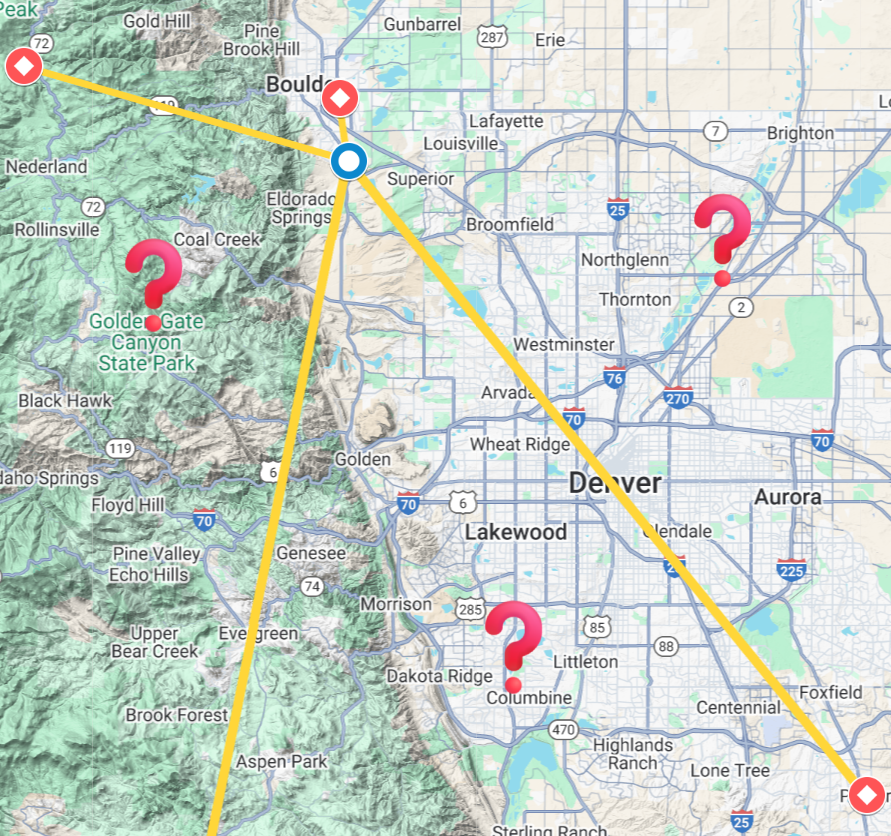
\includegraphics[height=0.4\textheight]{img/zephyr_map_q.png}
        \end{column}
    \end{columns}
\end{frame}